\subsection{Route Filtering} \label{sec:routefilter}
\begin{figure}[h!] 
	\centering
	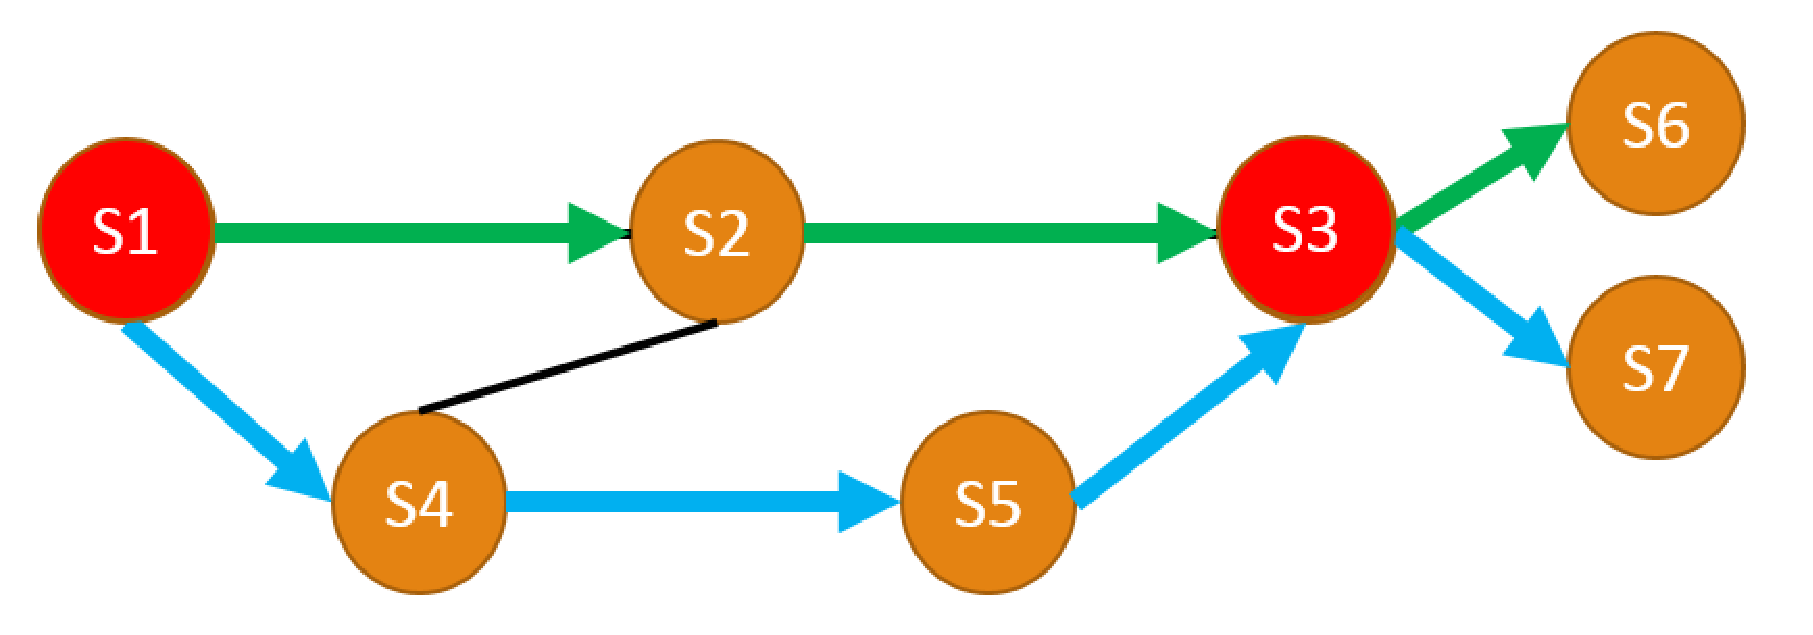
\includegraphics[width=\columnwidth]{figures/diamond.eps}
	\caption{Data plane example which requires route-filtering} \label{fig:diamond}
\end{figure}
Pure ARCs cannot be synthesized for all data planes. Consider the data
plane in \Cref{fig:diamond}. 
There exists no solution to the edge weights for this data plane. This is because 
there are two disjoint shortest paths connecting $s1$ and $s3$, and each path will have 
constraints
asserting it is the shortest of the two paths. 

How can we synthesize an ARC for the above scenario? 
If we could disable the edge
$s1 \rightarrow s4$ for destination $s6$, then we can synthesize ARC weights
such that path $s1 \rightarrow s2 \rightarrow s3$ is taken to reach $s6$, 
even if the actual shortest path
from $s1$ to $s3$ is via $s4$ and $s5$. 
If a route-filter is added on switch $s4$, $s4$ 
will not advertise a route for $s6$ to $s1$, so 
$s1$ will forward to $s2$ and not to $s4$
to reach $s6$. The forwarding of packets destined
for $s7$ are not affected, and they will be sent from
$s1$ to $s4$ as it is the shortest path.
Thus, by incorporating route-filters, we can
disable certain links in the topology 
for specific destinations, and increase the 
expressiveness of our synthesis. \kausik{expressiveness
may not be the right term.}

Given a data plane, we can trivially find an 
ARC enforcing the data plane by placing 
route-filters on all alternate paths (ref to fig)
except the shortest paths of the DAGs. However, this
ARC lacks the resilience properties we desire in
distributed control planes. Moreover, this ARC would be
0-resilient, and a single link failure can sever 
connectivity among endpoints (as all alternate paths
are blocked by route-filters). 

\subsubsection{Linear Equations with Route-Filters}
Write about modified rf Linear Equations.

\subsubsection{Diamond Elimination}
We define the structure shown in \Cref{fig:diamond}
as a \emph{diamond}. Formally,
consider two switches $s$ (the source of the diamond) 
and $t$ (the target of the diamond).
There exist two different destination DAGs with 
paths starting from $s$ such that they forward t
o different switches from $s$  
and these divergent paths from $s$ converge
at the switch $t$ first. A diamond is 
a reason for the ARC synthesis resulting in no
solution. 
\begin{theorem} \label{thm:diamond}
If the data plane contains a diamond, then no pure ARC  
can be synthesized for the data plane.
\end{theorem}
Thus, to generate an ARC, we need route-filters
to eliminate the diamond structures. Consider
the diamond in \Cref{fig:diamond}. There are two choices
of route-filters: the $s1-s2$ edge for destination $s7$ 
and the $s1-s4$ edge for destination $s6$, out of which,
at least one filter is required to eliminate the 
inconsistency in the linear equations due to the diamond.
Thus, we find all diamonds for all pairs of destination
DAGs (this is done in polynomial time) and assign a filter
to one of the two edges at the source of each diamond. 

\subsubsection{Unsat-Core Learning Approach}
The converse of \thmref{thm:diamond} does not hold, i.e.,
there exists data planes without diamonds for which
we cannot synthesize a pure ARC. We illustrate one example
in \Cref{}. (example figure and why inconsistent). 

\kausik{This para may need more work.}
Characterising the properties of structures causing
inconsistencies in the ARC synthesis is a tough algorithmic
problem and is an interesting study of future work. An
efficient algorithm to find the structures causing 
inconsistencies can be used to assign route-filters in an
optimal manner, thus maximizing resilience of the control plane.

Modern LP-solvers have efficient procedures to return an
unsatisfiable core, also called IIS (Irreducible Inconsistent Subsystem)
~\cite{iis}. Formally, an IIS is a subset of constraints such that
if all constraints except those in the IIS are removed, the set of
linear equations is still inconsistent. However, further removing 
any one constraint of the IIS produces an consistent result. 

A route-filter effectively removes certain equations. 
Consider the example in \cref{fig:diamond}, where we choose
a route-filter such that link $s1 \rightarrow s4$ is disabled for
destination $s6$. While generating \Cref{eq:uniq}, we will not
generate the following equation: 
\begin{eqnarray}
E(s1, s2) + E(s2, s3) < E(s1, s4) + D(s4, s3) \nonumber
\end{eqnarray} 